\begin{figure}[htbp]
\centering
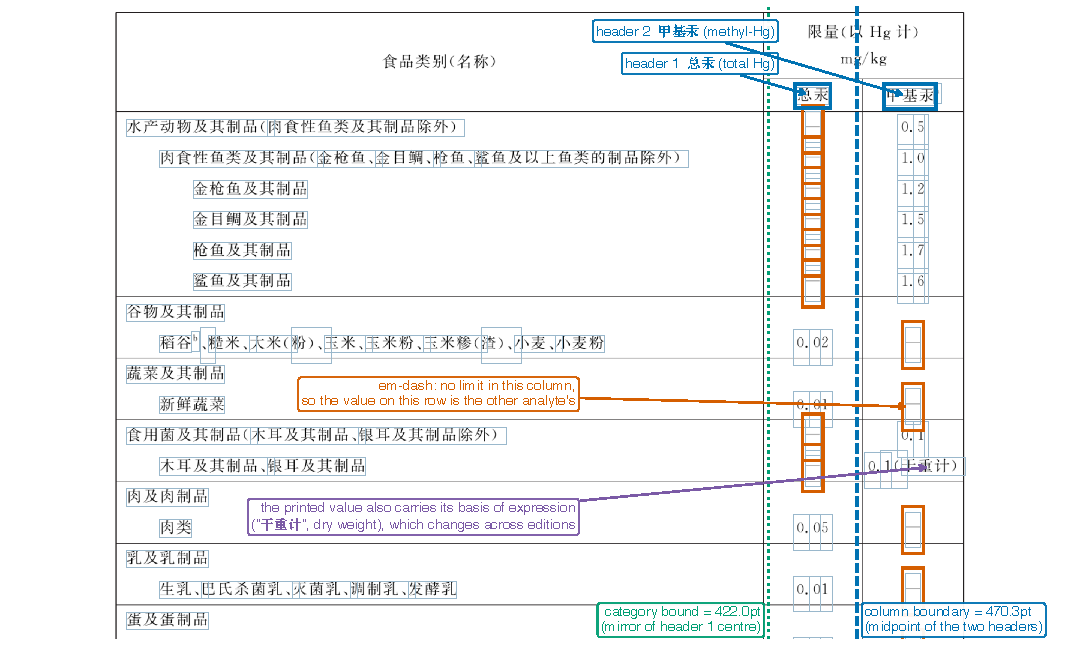
\includegraphics[width=\textwidth]{Results/fig/fig1ColumnAssignment.pdf}
\caption{Column assignment in the two-column tables. The mercury table of GB 2762-2022 is rendered with word bounding boxes. Its two analyte headers set the value-column boundary at 470.3 pt, and the inferred category boundary is 422.0 pt. Both are derived per page. Each row has a value in one column and an em-dash in the other, so the dash position assigns the value to an analyte. The same page also shows that an equal printed value can carry a different basis of expression.}
\label{fig1ColumnAssignment}
\end{figure}
